
\begin{figure}
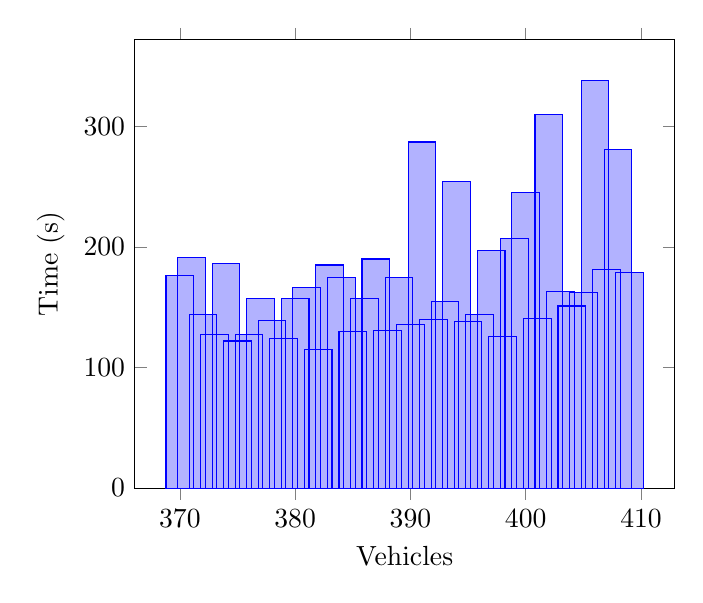
\begin{tikzpicture}
\begin{axis}[
legend style={anchor=west},
xlabel=Vehicles,
ylabel=Time (s),
ymin=0,
ybar,
]
\addplot coordinates {
(407, 181)
(406, 338)
(405, 162)
(403, 163)
(402, 310)
(401, 141)
(400, 245)
(409, 179)
(379, 124)
(378, 139)
(370, 176)
(373, 127)
(375, 122)
(374, 186)
(393, 155)
(392, 140)
(391, 287)
(397, 197)
(396, 144)
(395, 138)
(394, 254)
(398, 126)
(380, 157)
(381, 166)
(382, 115)
(383, 185)
(384, 175)
(385, 130)
(386, 157)
(387, 190)
(388, 131)
(389, 175)
(404, 151)
(408, 281)
(371, 191)
(377, 157)
(376, 127)
(390, 136)
(372, 144)
(399, 207)
};

\end{axis}
\end{tikzpicture}
\label{tik:time:100:56}
\caption{100 percent diving with GSC on route $56$}
\end{figure}
